\subsection{形体分析法}
形体分析法是从能够反映物体形状特征的视图出发,分析该物体由哪几个部分组成,采用什么形式组合,然后运用视图投影规律,找出每个部分在其它视图上的投影,从而想象出各个部分所表达的基本形体的形状及各部分之间的相互位置关系,最后综合想象出整个物体的形状的方法。

下面以图所示的三视图来说明形体分析法看图的步骤。

一、看视图,分析物体的形体组成部分。运用形体分析法将视图分成3个部分,如图\ref{fig:kantu}所示。
\begin{figure}[htbp]
\centering
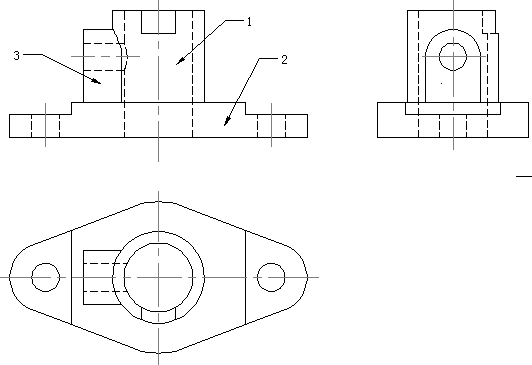
\includegraphics[scale=0.5]{kantu.png}
\caption{分析组成部分}\label{fig:kantu}
\end{figure}

二、找投影关系,想形体。从线框出发,从三视图中找出各个部分的投影,确定特征视图,想象形状。
\begin{figure}[htbp]
\centering
\subfloat[]{\label{fig:kantu3}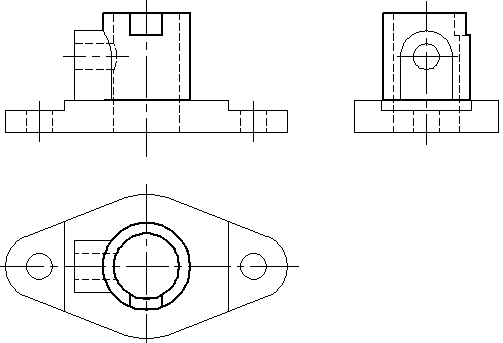
\includegraphics[scale=0.4]{kantu3.png}}\hspace{30pt}
\subfloat[]{\label{fig:kantu4}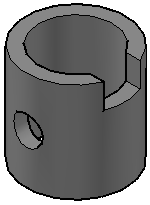
\includegraphics[scale=0.6]{kantu4.png}}
\caption{套筒部分}
\end{figure}

\begin{figure}[htbp]
\centering
\subfloat[]{\label{fig:kantu1}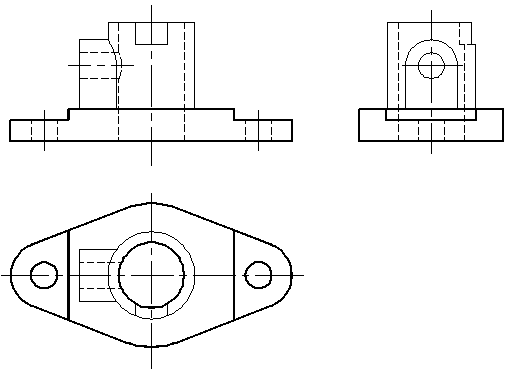
\includegraphics[scale=0.4]{kantu1.png}}\hspace{30pt}
\subfloat[]{\label{fig:kantu2}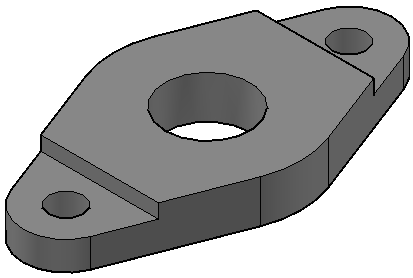
\includegraphics[scale=0.3]{kantu2.png}}
\caption{底板部分}
\end{figure}
图\ref{fig:kantu3}所示,粗实线为第1部分套筒的三视图,从三视图可知,该套筒上前部分开有缺口,左中部分开有孔,如图\ref{fig:kantu4}所示。

图\ref{fig:kantu1}所示,粗实线为第2部分底板的三视图,从三视图可知,该底板整体上为一凸台,并有三个通孔,如图\ref{fig:kantu2}所示。

图\ref{fig:kantu5}所示,粗实线为第三部分凸台的三视图,从三视可知,该凸台由四棱体和半圆柱构成,并且右边被圆柱曲面切割,上半部分有一通孔, 如图\ref{fig:kantu6}所示。

\begin{figure}[htbp]
\centering
\subfloat[]{\label{fig:kantu5}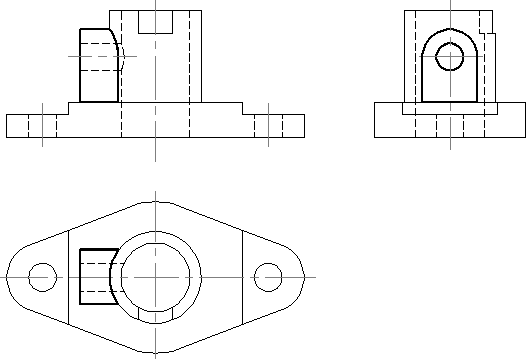
\includegraphics[scale=0.4]{kantu5.png}}\hspace{30pt}
\subfloat[]{\label{fig:kantu6}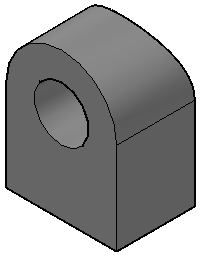
\includegraphics[scale=0.3]{kantu6.png}}
\caption{凸台部分}
\end{figure}

三、明确位置和连接关系。在想象出各部分形体后,需要利用位置特征视图,确定各部分的位置和表面连接关系。确定位置关系和表面连接关系通常是难以截然分开的,需要进行综合考虑。图\ref{fig:kantu}所示,第1部分位于第2部分上面正中心位置,第3部分位于第2部分上面,位于第1部分左边并与之相贯。

四、综合分析,想象整体。将上面各个部分的形体和位置分析综合起,便可以想角出整个形体,如图\ref{fig:kantu7}所示。
\begin{figure}[htbp]
\centering
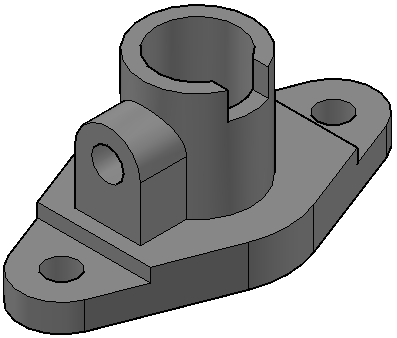
\includegraphics[scale=1]{kantu7.png}
\caption{支座空间形体}\label{fig:kantu7}
\end{figure}
\endinput